% The efficacy of your chosen model will be one of the main factors behind choosing it as your approach and dismissing alternatives.
% This can be demonstrated by showing a range of performance metrics for the model you have chosen as well as for the alternatives considered
% Justify your choice of metrics stating why they are appropriate for this particular implementation of machine learning
% It may be easiest to present these metrics and methods in a tabular format

\section{Implementation and performance metrics}

I trained an \textbf{autoencoder} \cite{DBLP:journals/corr/abs-2003-05991,DBLP:journals/corr/abs-2201-03898}
to learn the Passport tags' latent features and reduce the encoded vectors' size.
The autoencoder is an encoder-decoder neural network, a self-supervised model capable of capturing non-linearity from the data.
I used the ``undercomplete'' variant, which constrains the number of nodes in the hidden layers, creating a ``bottleneck''
of information flow through the network.
This architecture is a form of \textit{regularisation} that forces the model to learn latent attributes from the input
while reconstructing it with minimal loss. Ultimately, it helps prevent the model from overfitting the training dataset by indexing it like a caching layer.
The autoencoder has a symmetrical architecture composed by the \textit{encoder} and the \textit{decoder} sub-networks,
with a bottleneck layer in the middle also known as \textit{code} [figure \ref{fig:autoencoder} and \ref{fig:dataset_encoded}].

\begin{figure}[H]
  \centering
  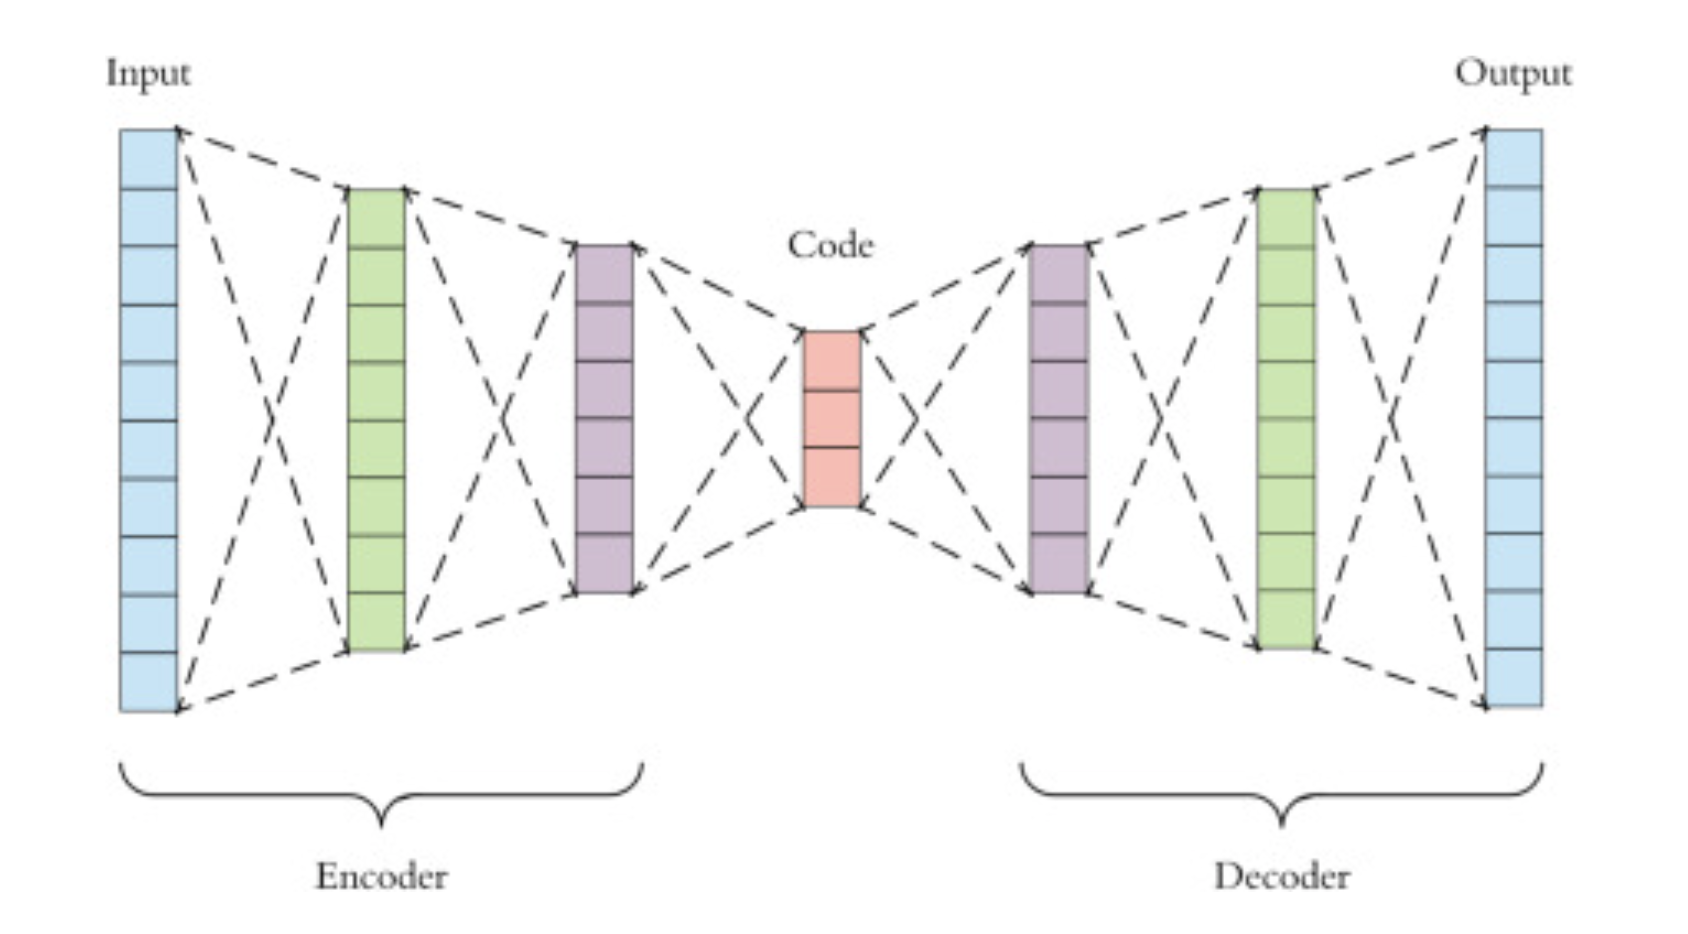
\includegraphics[scale=0.4]{autoencoder}
  \caption{Undercomplete autoencoder architecture}
  \label{fig:autoencoder}
\end{figure}

I extracted the trained \textit{encoder} segment of the network to compress the one-hot encoded high-dimensional sparse array into
a lower-dimensional and denser representation called \textit{embeddings} \cite{GoogleForDevelopers:Embeddings} [code \ref{lst:embeddings}].
This technique solved the curse of dimensionality and the data sparsity problems and improved the calculation
complexity and the quality of the recommendations at inference time [code \ref{lst:cosine_similarity}].

\subsection{Hyperparameters}

Some of the hyperparameters were decided based on the nature of the problem.
The input data was a tensor of zeros and ones, and the network's main objective was to reconstruct the output with minimal loss.
I used the \textit{Sigmoid} activation function for the output layer and \textit{binary cross-entropy} as a loss function
to allow the network to minimise the reconstruction error, pushing the values of the output between zero and one.
The minimisation of the reconstruction error was the reason for using \textit{binary cross-entropy} as the performance metric.
I did not use the \textit{SoftMax} activation function for the output layer because every node needed to be able to assume those values.
I did not use any residual-based loss function either because the penalty for wrong predictions
(i.e., when the X-axis value is close to zero) is not as significant as for the binary cross-entropy loss.
Because the slope of the derivative in this region is not steep enough, it also affects the step size during backpropagation [figure \ref{fig:loss_comparison}].
The negative log loss was the best option because it heavily penalised significant differences between $y$ and $\hat{y}$,
with a natural logarithmic progression.

\begin{figure}[H]
  \centering
  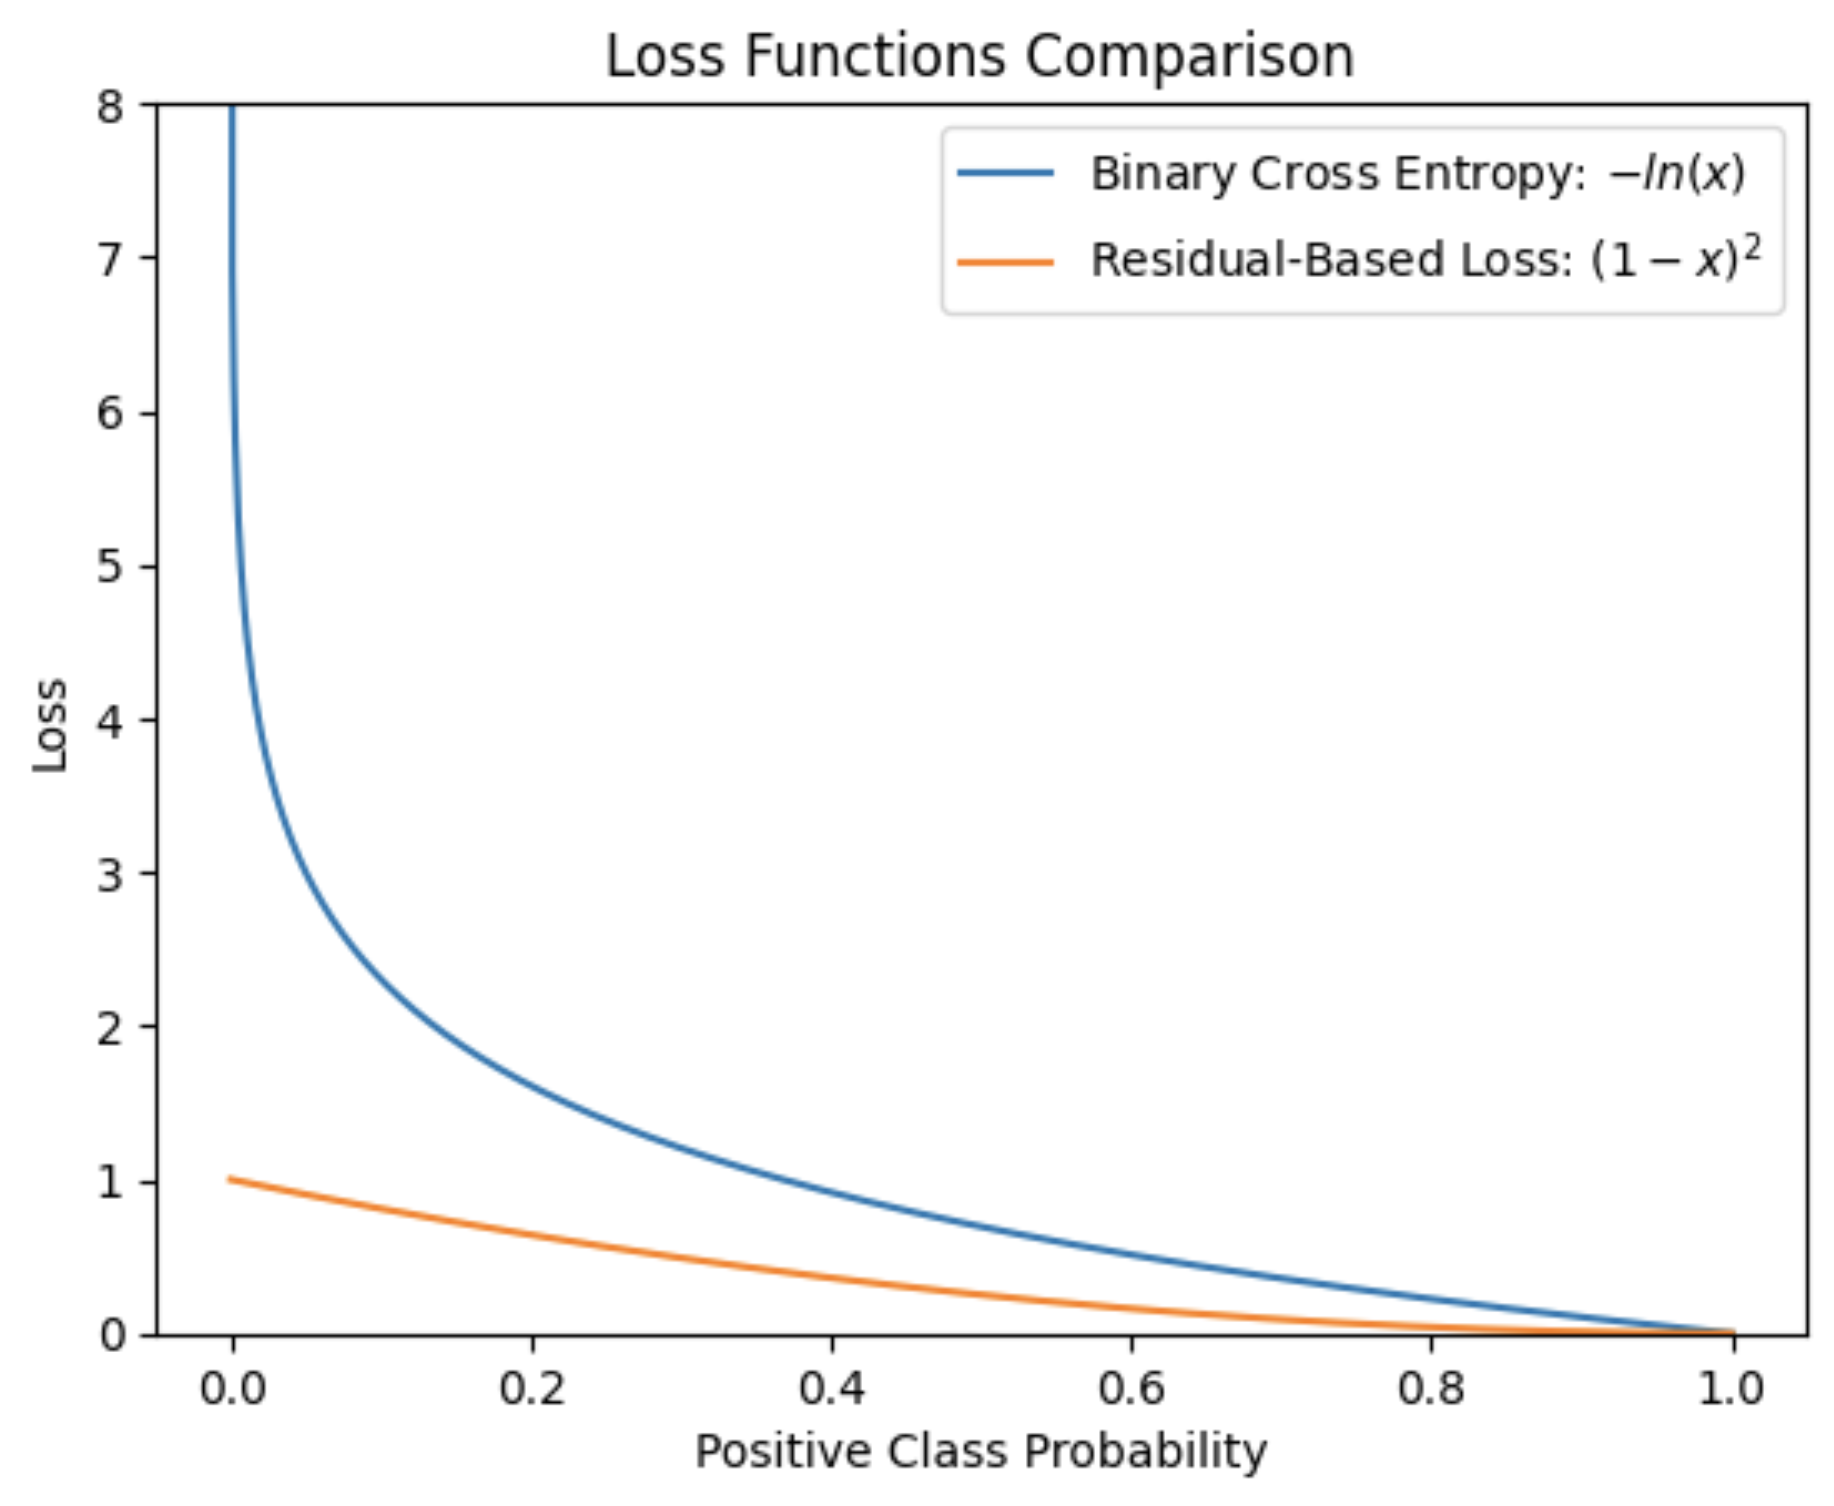
\includegraphics[scale=0.2]{loss_comparison}
  \caption{Comparison between Binary Cross-Entropy and Square Residuals loss functions}
  \label{fig:loss_comparison}
\end{figure}

I used the \textit{Rectified Linear Unit (ReLU)} as an activation function for the hidden layers
while testing other variants like \textit{Leaky ReLU (LReLU)} and \textit{Parametric ReLU (PReLU)},
but without any relevant improvements in performance.
Some other hyperparameters were:

\begin{itemize}
  \item \textbf{optimizer:} \verb|Adam|
  \item \textbf{number\_of\_epochs:} \verb|100|
  \item \textbf{batch\_size:} \verb|300|
  \item \textbf{dropout\_rate:} \verb|0.2|
  \item \textbf{early\_stopping\_patience:} \verb|10|
  \item \textbf{early\_stopping\_monitoring:} \verb|binary cross-entropy| on the validation set
  \item \textbf{data\_split\_ratio:} \verb|80% training, 10% validation, 10% test|
\end{itemize}

I used a ``Bandit-based'' approach called \textit{Hyperband} \cite{DBLP:journals/corr/LiJDRT16} to optimise the remaining hyperparameters
[codes \ref{lst:hyperband}, \ref{lst:hyperband_search}].
It improves upon \textit{Random Search} by running fewer epochs on the randomly sampled set of parameters
and moving on to the next stage by only testing the best-performing ones, returning a ranked list of the best hyperparameter sets.
The hyperparameters considered by Hyperband were:

\begin{itemize}
  \item the number of hidden layers
  \item the embedding size
  \item the learning rate
  \item whether to use dropout
  \item whether to use batch normalisation
\end{itemize}

The number of hidden layers was a positive odd integer $N > 0$.
The network had the encoder and decoder with $N-1$ layers and the bottleneck layer in the middle.
If the value were $1$, the network would only have the bottleneck.

The number of nodes per layer was a positive integer $N > 0$.
Unfortunately, the number of combinations was too high to be meaningfully optimised.
To reduce the complexity, I decided to limit the values of this hyperparameter to a progression of integer divisions by 2,
starting from the number of nodes in the input layer.
Each hidden layer in the encoder could have half the number of nodes compared to the previous one and double the amount of the successive one
(and \textit{vice versa} for the decoder), except for the layers adjacent to the input and output.
In that case, they could assume any progression value depending on the number of hidden layers and embedding size.

For example, because I had 8982 nodes in input, the progression of layer dimensions
was \verb|[4491, 2245, 1122, 561, 280, 140, ...]|.
The embedding size was also bound to assume one of these values, which would determine
the maximum number of hidden layers allowed.
Therefore, a network with \verb|5| hidden layers and an embedding size of \verb|280|
would have had the following configuration: \verb|8982 -> 1122 -> 561 -> 280 -> 561 -> 1122 -> 8982|.
While a network with \verb|3| hidden layers but an embedding size of \verb|2245| would have had the following configuration:
\verb|8982 -> 4491 -> 2245 -> 4491 -> 8982|, representing the maximum extension of the progression.

\subsection{Training and validation}

To improve and assess the ability of the model to \textit{generalise} on unseen data, I randomly shuffled the dataset and split
it into three chunks: training, validation and test [code \ref{lst:data_splitting}].
The training phase took \verb|20h 55m 11s| on Sagemaker to tune the hyperparameters,
returning the following best values:

\begin{itemize}
  \item \textbf{hidden\_layers:} \verb|1|
  \item \textbf{embeddings\_size:} \verb|560|
  \item \textbf{batch\_norm:} \verb|False|
  \item \textbf{dropout:} \verb|True|
  \item \textbf{learning\_rate:} \verb|0.01|
\end{itemize}

The trained model had \verb|8982| nodes for the input and output layers - which corresponded to the size of
the one-hot encoded array - and \verb|560| nodes for the bottleneck layer, with a total of \verb|10069382 (38.41 MB)|
parameters [figure \ref{fig:model_summary}]

\begin{figure}[H]
  \centering
  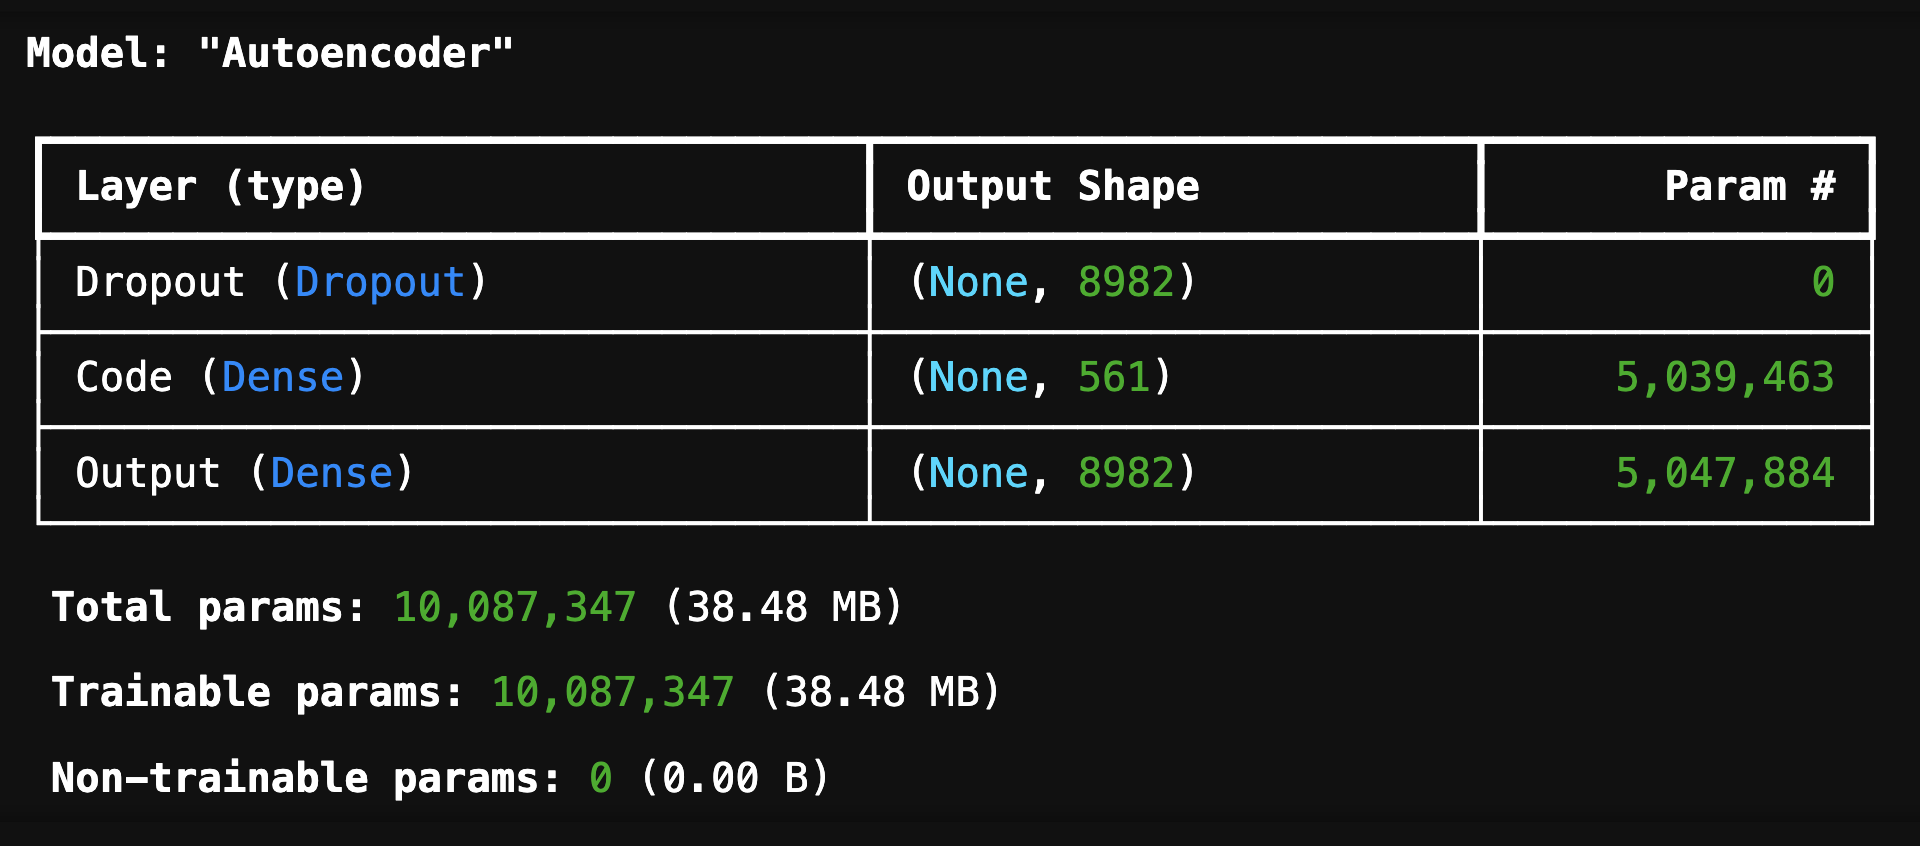
\includegraphics[scale=0.5]{model_summary}
  \caption{Autoencoder model summary}
  \label{fig:model_summary}
\end{figure}

Training completed with a reconstruction error of \verb|0.0002933757205028087| on the validation set
[figure \ref{fig:binary_cross_entropy}] [codes \ref{lst:model_retraining},\ref{lst:loss_visualisation}].

\begin{figure}[H]
  \centering
  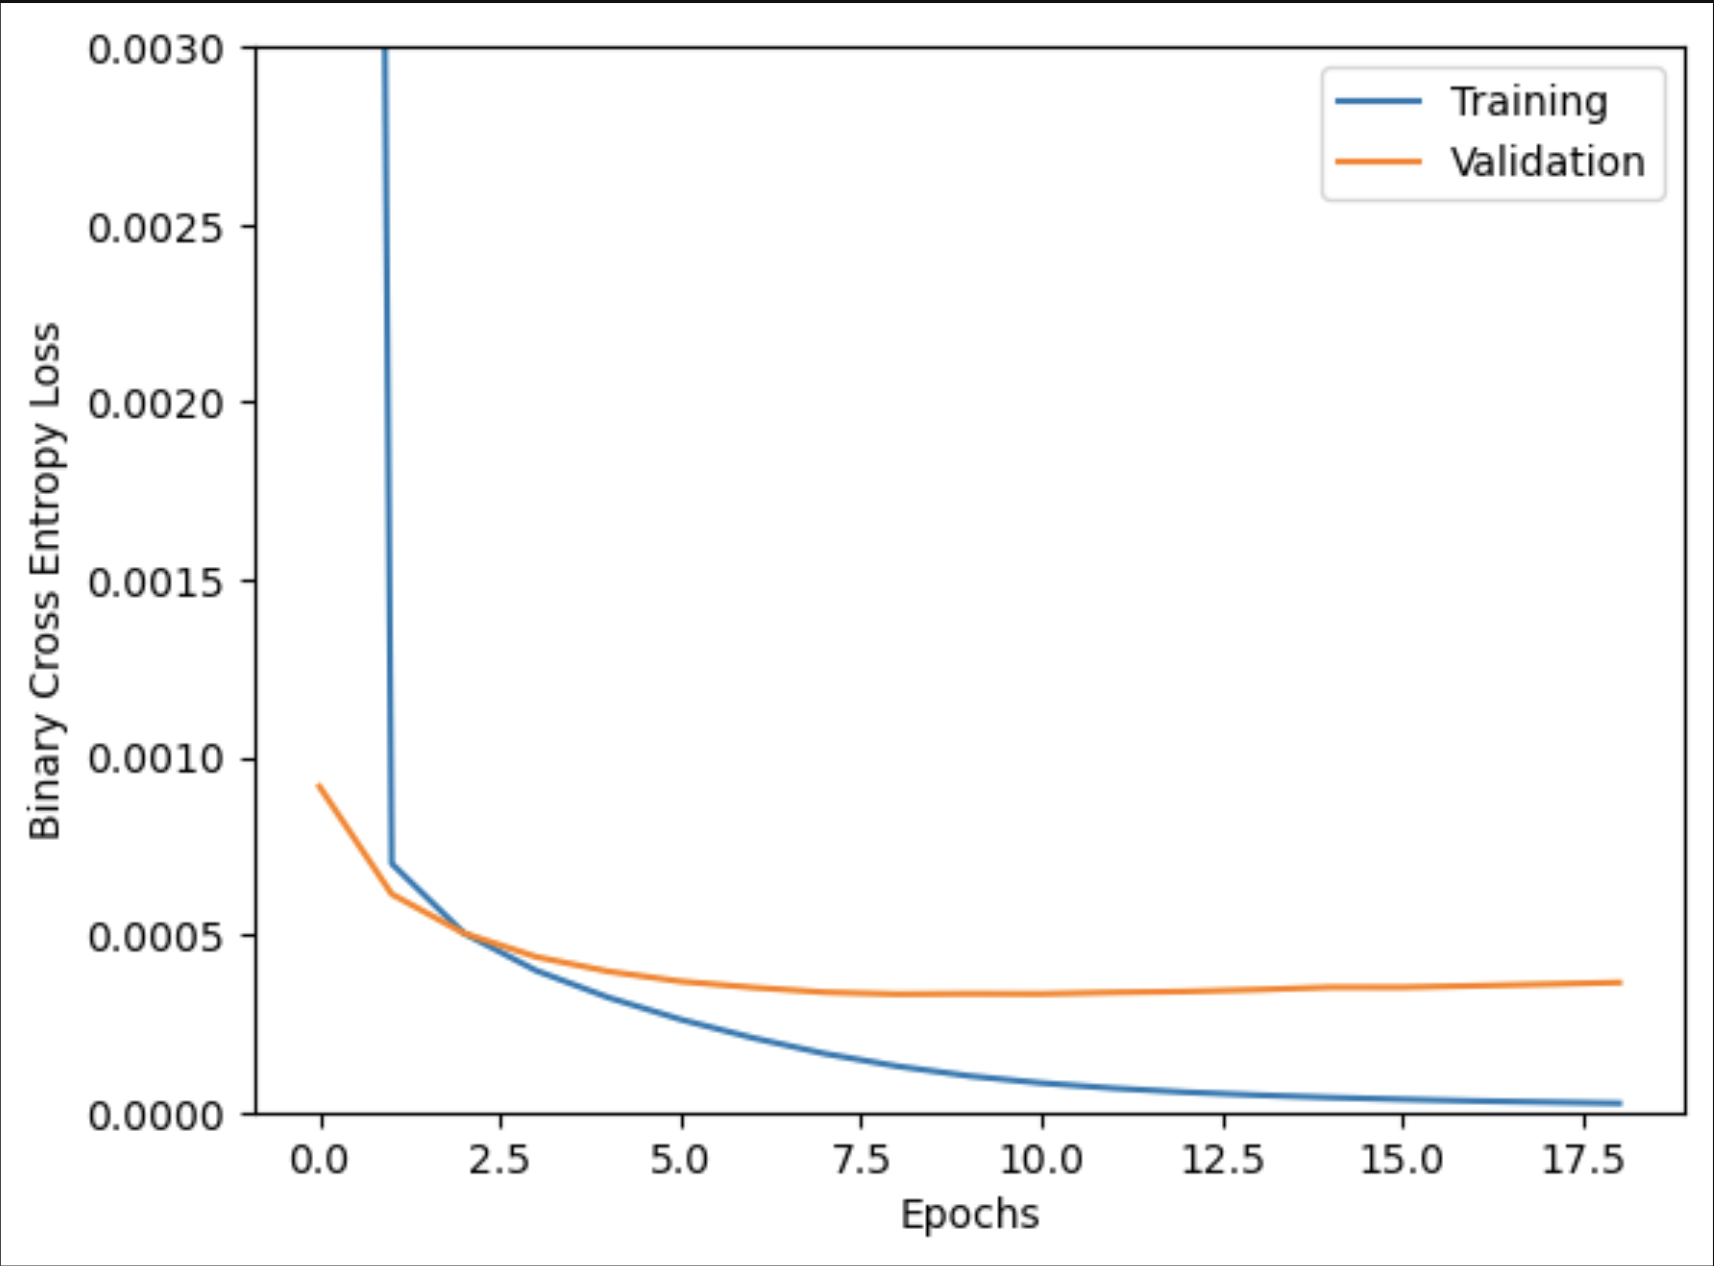
\includegraphics[scale=0.4]{binary_cross_entropy}
  \caption{Binary cross-entropy loss on the training and validation sets}
  \label{fig:binary_cross_entropy}
\end{figure}

\subsection{Strengths and Weaknesses}

The strength of this approach was the efficient use of space and the fast inference time.
The space scaled linearly with respect to the input size to store the embeddings [figure \ref{fig:embeddings}]
and quadratically to store the similarity scores [figure \ref{fig:similarity_scores}].

\begin{figure}[H]
  \centering
  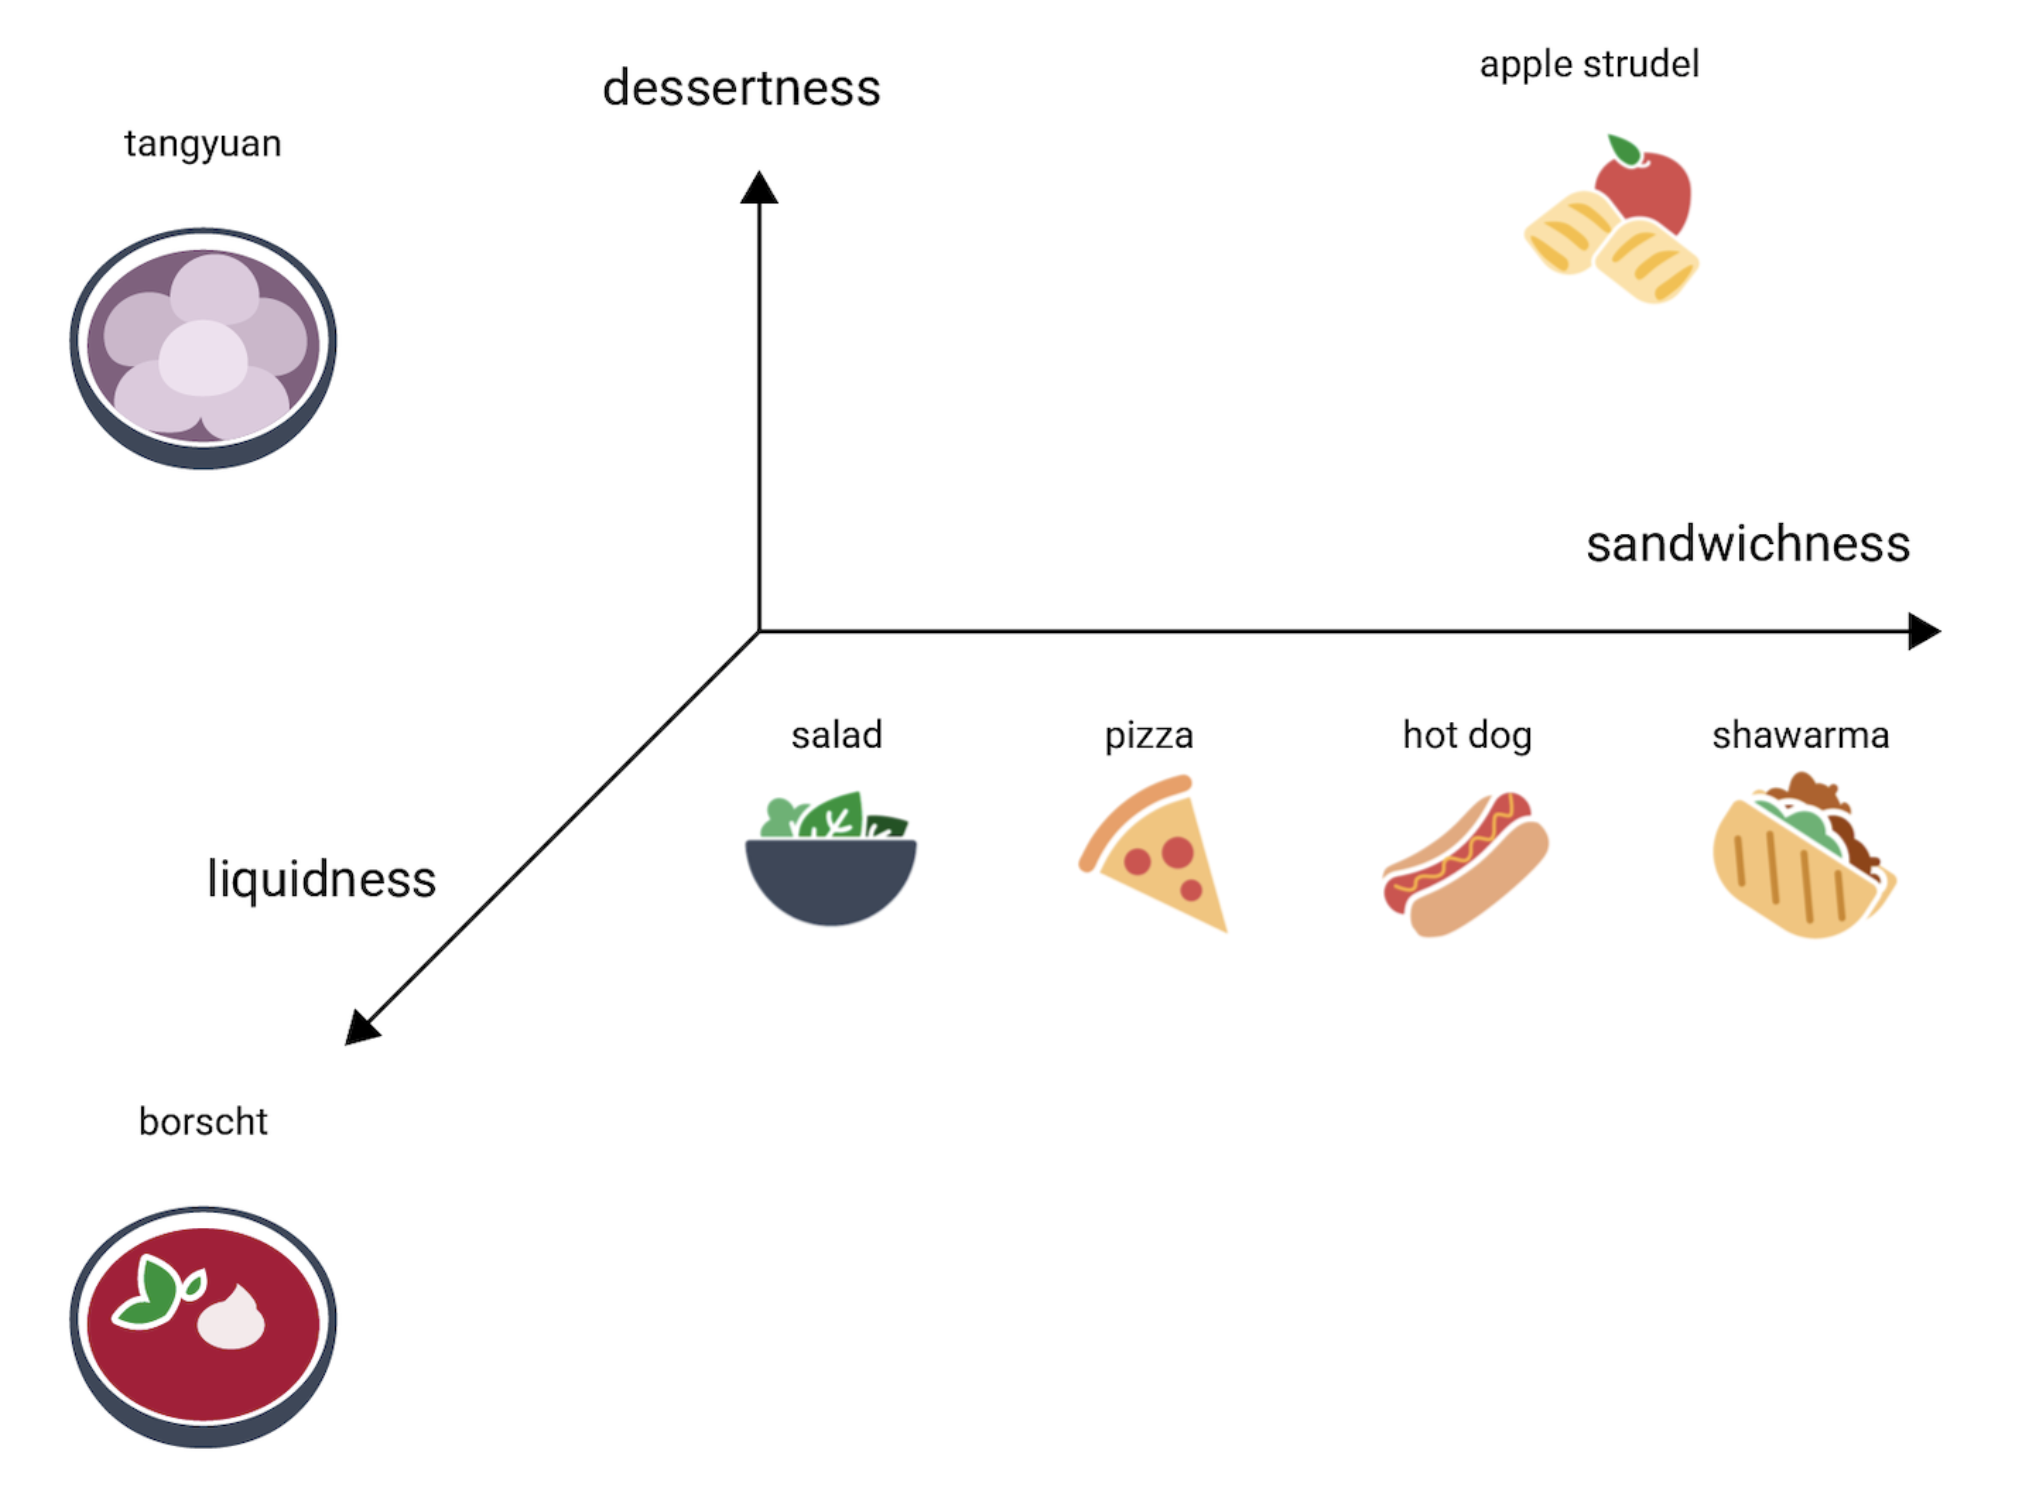
\includegraphics[scale=0.26]{embeddings}
  \caption{Embeddings dataset}
  \label{fig:embeddings}
\end{figure}

\begin{figure}[H]
  \centering
  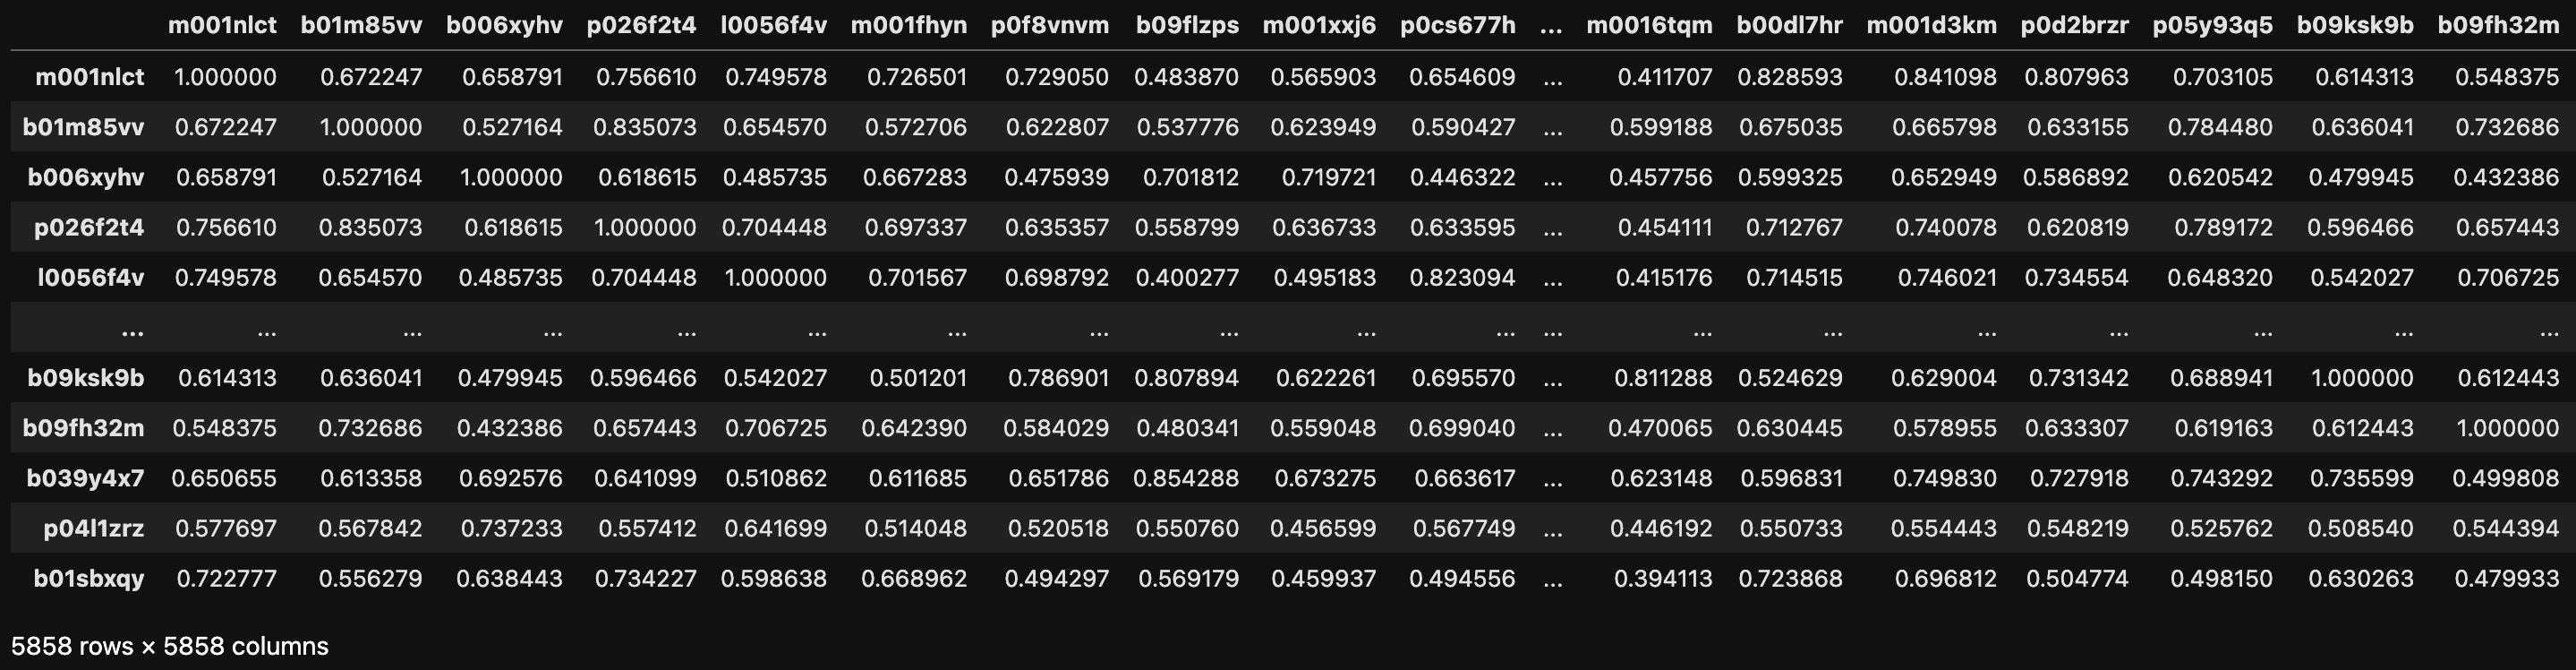
\includegraphics[scale=0.26]{similarity_scores}
  \caption{Similarity scores dataset}
  \label{fig:similarity_scores}
\end{figure}

Hyperparameter tuning took quite some time, but this drawback was compensated by the fact that training was performed offline
while the recommendations were cached and served instantly.
In addition, retraining could be scheduled to cover the new programmes added to the iPlayer catalogue and the unavailable ones being removed
[figures \ref{fig:catalogue_pids_added}, \ref{fig:catalogue_pids_dropped}].

The main weakness was the model's interpretability.
The autoencoder is a black box by definition, and using embeddings to calculate the similarity just worsened the problem.
It was unlikely to interpret which of the tags influenced the ranking in the top-K recommendation by untangling the weights and biases of the neural network,
so I analysed the composition and distribution of the tags of the recommended programs as an alternative.
